\section{Exemple d'application à un cas urbain}

Après avoir utilisé le cas-test Beaune pour tester plusieurs aspects de l'algorithme d'estimation, nous travaillons ici dans un cadre différent, qui est celui du milieu urbain. Plusieurs nouveaux facteurs d'incertitude sont ainsi introduits, et le but de ce paragraphe est d'examiner les résultats de l'AMIS dans un contexte à forte complexité.\\

\subsection{Présentation du cas-test}

Nous considérons désormais un cas-test en milieu urbain caractérisé par la présence d'obstacles multiples et de géométries variées sur le domaine (bâtiments). Pour cela, on utilise une reconstitution du quartier parisien de l'Opéra (figure \ref{fig_opera_config}), qui comme pour le cas-test Beaune, a initialement été utilisé pour la validation de RetroSPRAY.\\



\begin{figure}[h!]
	\centering
	\begin{subfigure}[t]{0.5\textwidth}
		\centering
		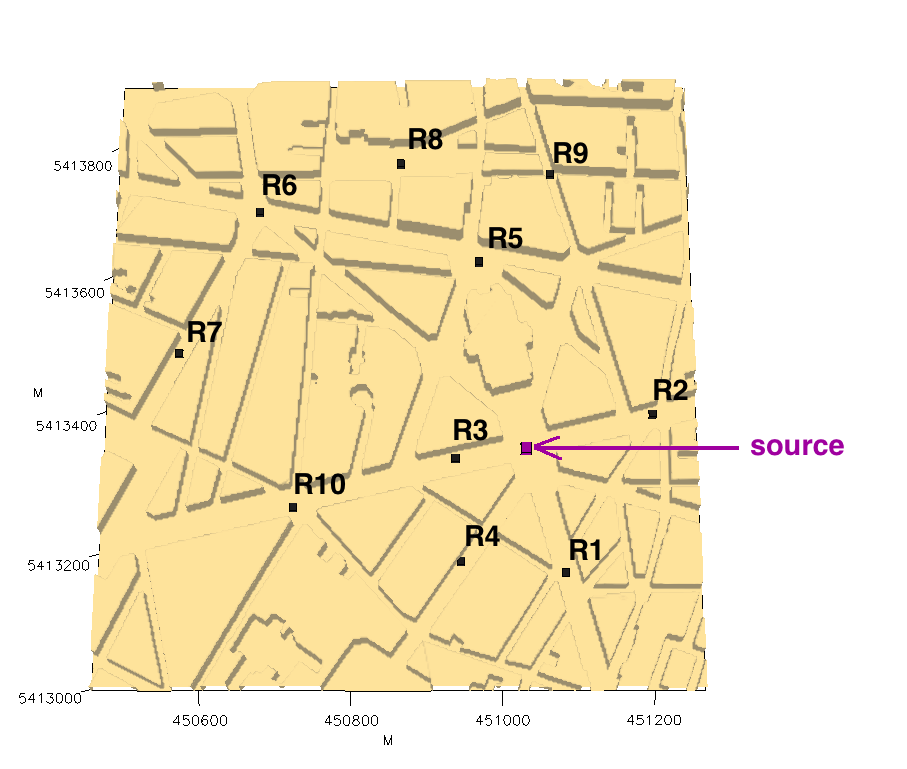
\includegraphics[width=1\textwidth]{opera_config_domaine.png}
		\caption{}
		\label{fig_opera_config}
	\end{subfigure}%
	\begin{subfigure}[t]{0.5\textwidth}
		\centering
		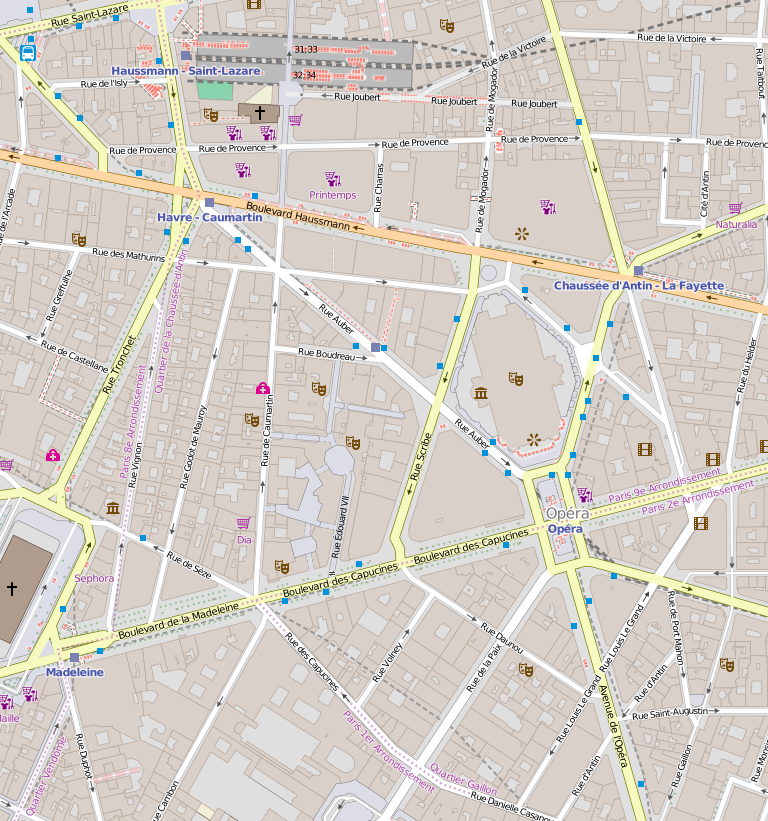
\includegraphics[width=0.75\textwidth]{opera_osm.png}
		\caption{}
		\label{fig_opera_carte}
	\end{subfigure}
	\caption{A gauche: illustration du milieu bâti, du réseau de capteurs (en noir) et de la source (en magenta) utilisés pour le cas-test Opéra. A droite: carte OpenStreetMap du cas-test Opéra.}
	\label{fig_opera_presentation}
\end{figure}

\subsubsection{Caractéristiques du domaine}
Le domaine couvre une surface de \SI{808}{\meter} $\times$ \SI{882}{\meter}, avec une source unique et un réseau de 10 capteurs, disposés de façon non-régulière. Pour la simulation, le domaine est discrétisé en une grille de $404 \times 441$ mailles, avec une résolution du maillage en $x$ et $y$ de \SI{2}{\meter}: il s'agit d'un espace d'étude plus petit que celui du cas-test Beaune, mais de résolution plus élevée, afin d'assurer une meilleure précision des calculs de dispersion atmosphérique en présence d'une topographie complexe. \\


\subsubsection{Paramètres météorologiques}
Pour ce cas-test, on choisit des paramètres météorologiques instationnaires, à savoir un vent de vitesse constante (\SI{3}{\meter \per \second}), mais dont la direction change toutes les heures:

\begin{center}
	\begin{tabular}{cccc}
		\centering
		Heure & 11:00 &  12:00 &  13:00\\ 
		\hline
		Direction du vent & $230\degres$ & $180\degres$ & $45\degres$
	\end{tabular} 
\end{center}

La combinaison de ces variations temporelles ainsi que de la présence d'obstacles sur le domaine fait que les champs de vent 3D diagnostiqués par SWIFT sont relativement complexes, comme l'illustre la figure \ref{fig_opera_vent}.

\begin{figure}[h!]
	\centering
	\begin{subfigure}[t]{0.5\textwidth}
		\centering
		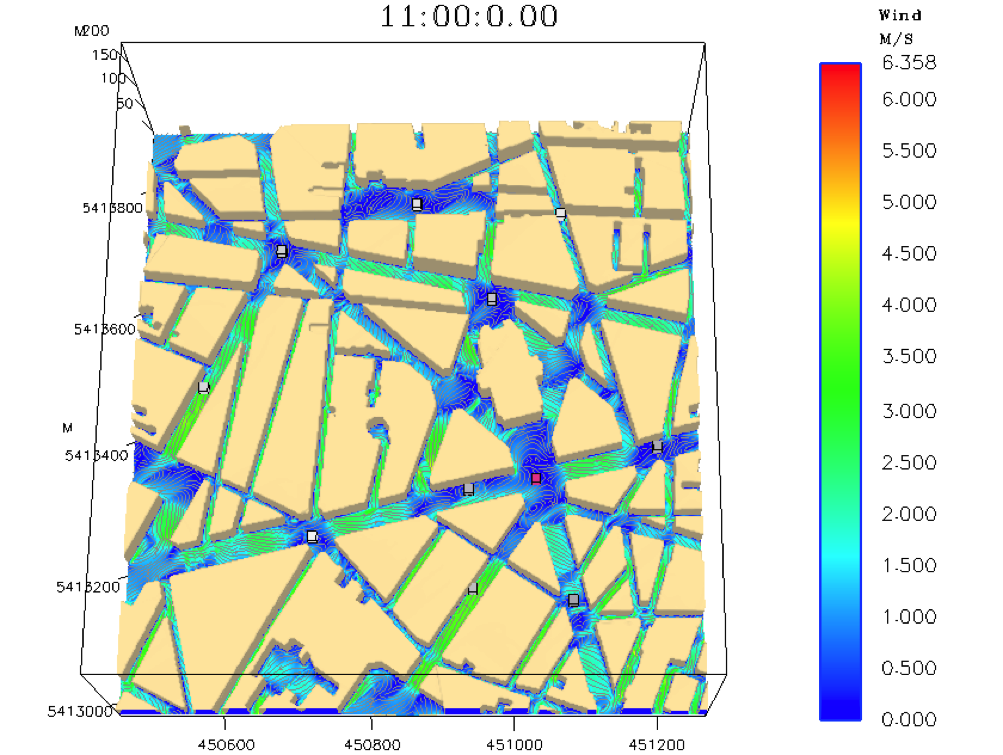
\includegraphics[width=1\textwidth]{opera_vent_11_00.png}
		\caption{}
		\label{opera_vent_11_00}
	\end{subfigure}%         	
	\begin{subfigure}[t]{0.5\textwidth}
		\centering
		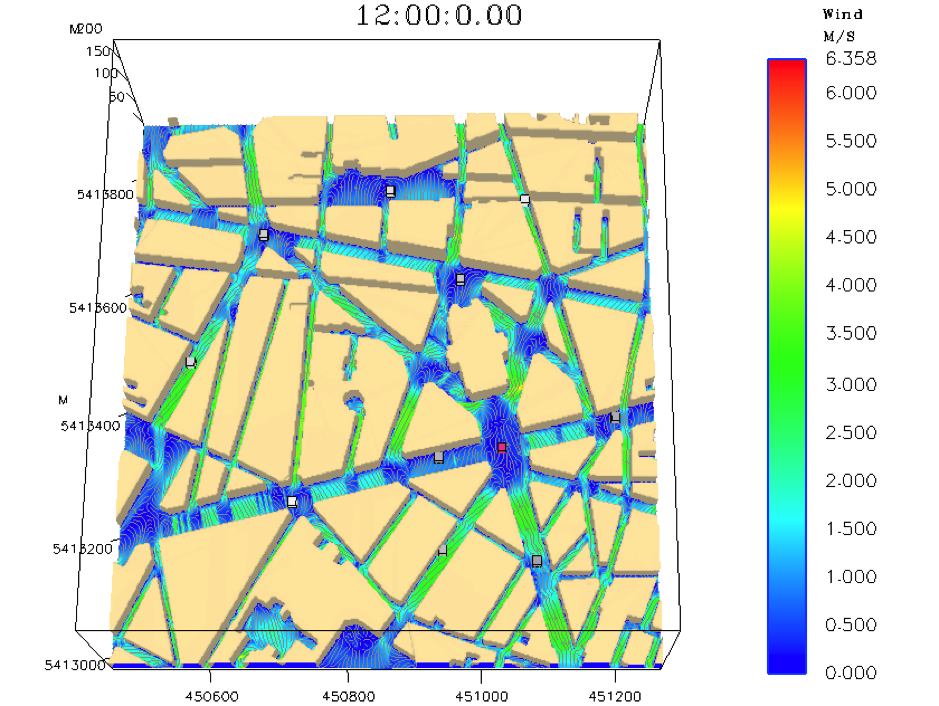
\includegraphics[width=1\textwidth]{opera_vent_12_00.png}
		\caption{}
		\label{opera_vent_12_00}
	\end{subfigure}
	\begin{subfigure}[t]{0.5\textwidth}
		\centering
		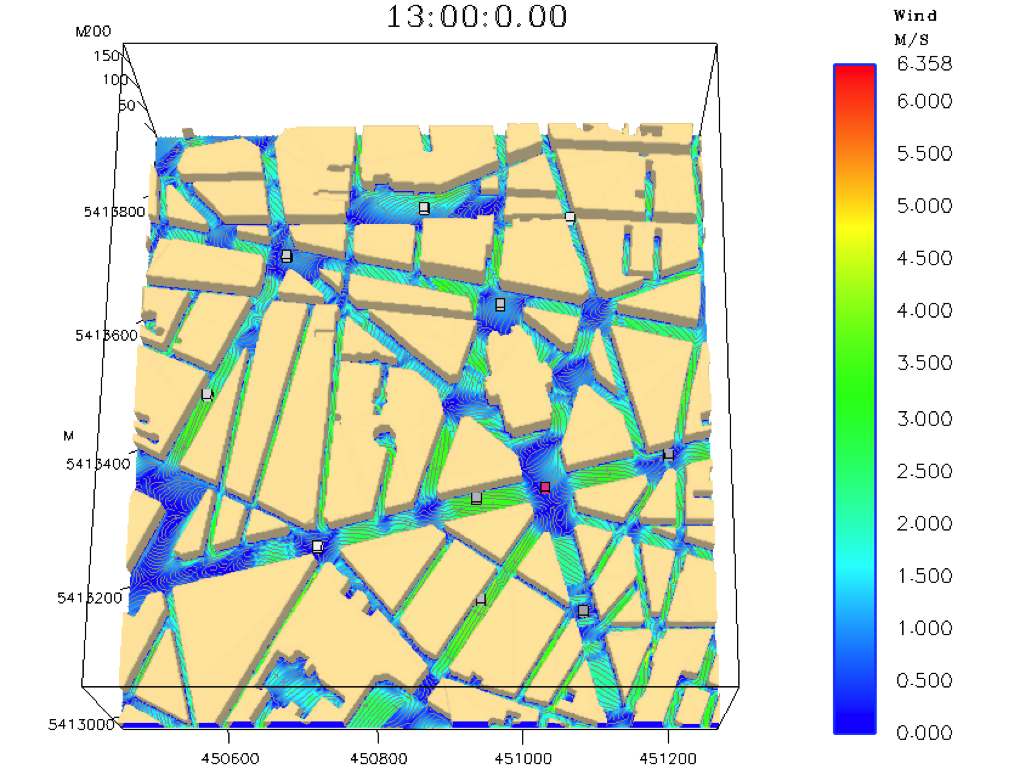
\includegraphics[width=1\textwidth]{opera_vent_13_00.png}
		\caption{}
		\label{opera_vent_13_00}
	\end{subfigure}%
	\caption{Champs de vent à \SI{2}{\meter} du sol produits par SWIFT aux trois échéances météorologiques considérées}
	\label{fig_opera_vent}
	
\end{figure}



\subsubsection{Capteurs, source et simulation des observations}
Le domaine contient un réseau de 10 capteurs, qui sont placés aux centres de diverses intersections de rues, ainsi que sur des places publiques. Ils sont situés à lune hauteur de 2m, et délivrent des valeurs de concentrations moyennées sur des plages de 5 minutes entre 11h35 et 13h.

La source est également située à 2m du sol, positionnée au niveau d'une grande intersection, et émet un rejet bref d'une durée de 10 minutes entre 12h10 et 12h20, avec un débit constant de $10^4$ unités/s. Ces caractéristiques se rapprochent de celles d'un rejet d'origine malveillante, par exemple suite à l'explosion d'une "bombe sale". 

On suit le même raisonnement que pour le cas-test Beaune et on simule le vecteur d'observations à partir d'une matrice source-récepteur \textit{backward} afin d'obtenir les mesures simulées de la figure \ref{fig_opera_obs}. Les dimensions de cette source sont celles d'une maille du domaine, à savoir un volume de 2m $\times$ 2m $\times$ 2m.

\begin{figure}[h!]
	\centering
	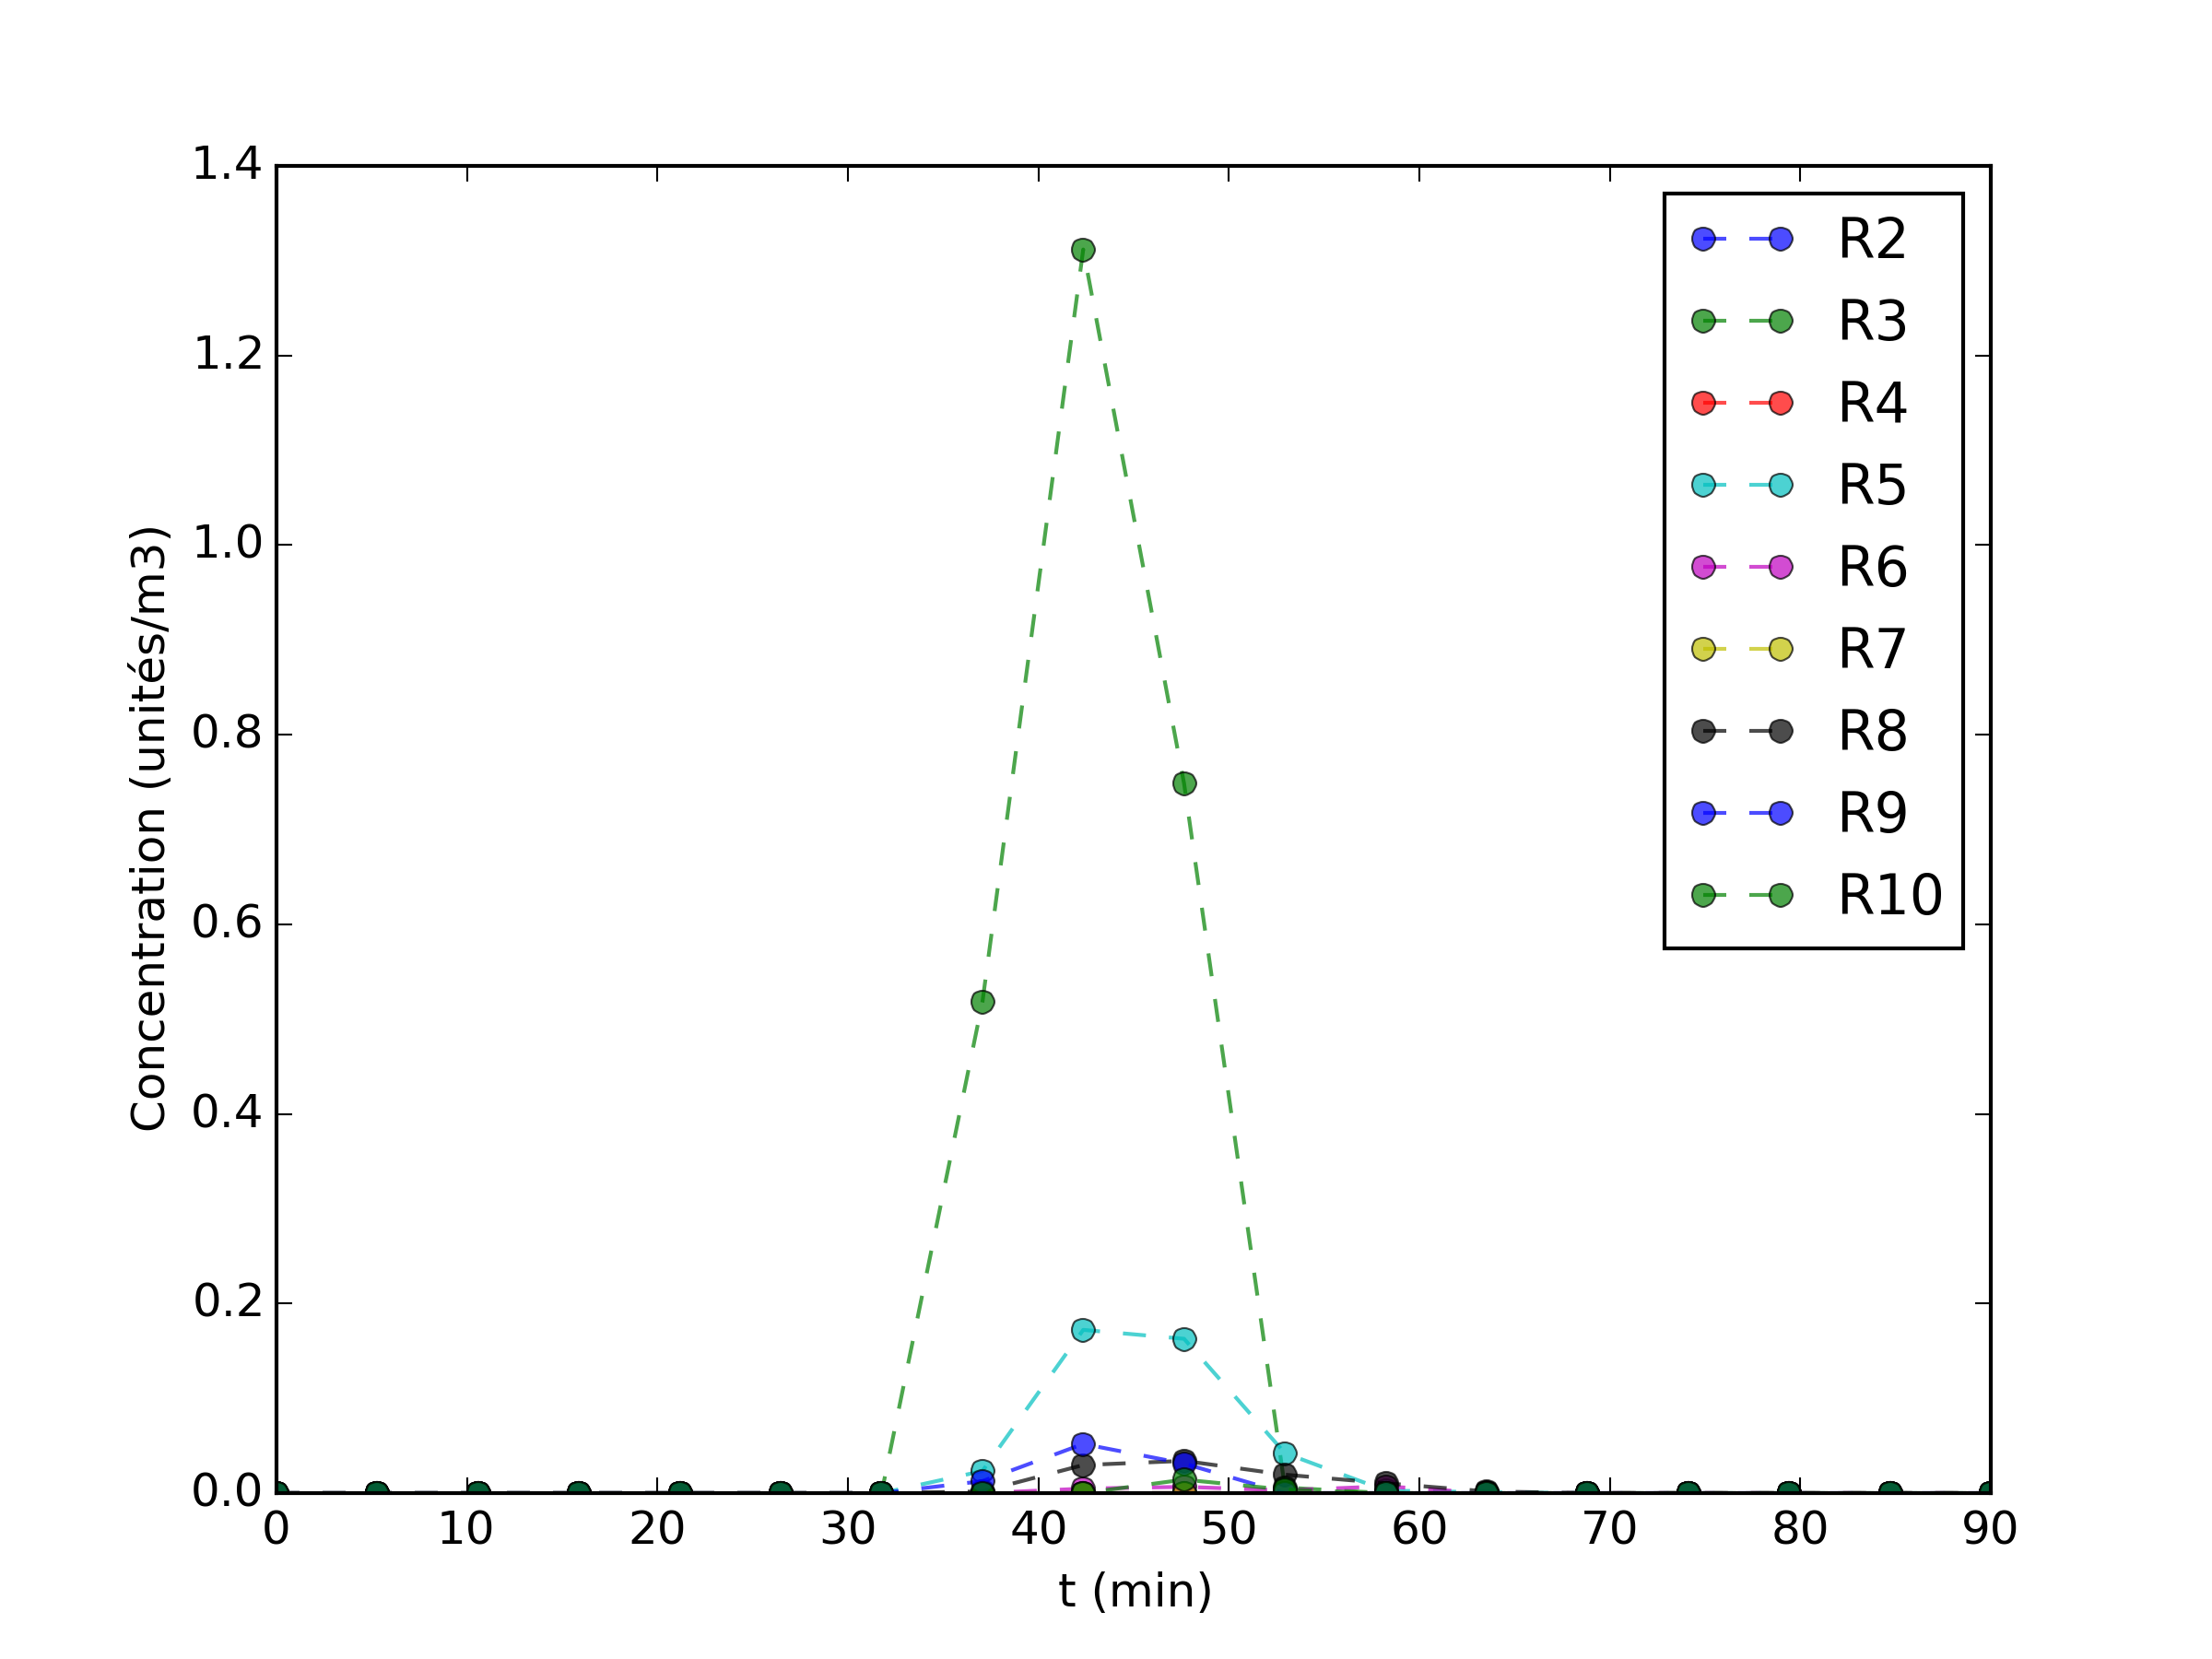
\includegraphics[width=0.8\textwidth]{concentrations_opera.png}
	\caption{Cas-test Opéra: concentrations mesurées aux capteurs}
	\label{fig_opera_obs}
\end{figure}

Etant donné la taille réduite du domaine ainsi que les conditions météorologiques instationnaires auquel le cas-test est confronté, on observe que malgré un nombre total de capteurs inférieur à celui du cas-test Beaune, la proportion de récepteurs mesurant une concentration non-nulle est ici plus élevée.


\subsection{Initialisation optimisée de la loi de proposition}

Avec le cas-test Opéra, il est vite apparu que sans apport préalable d'information, l'algorithme aurait des difficultés à converger vers une solution correcte étant donné la complexité du domaine. Une procédure préliminaire a donc été mise en place sur l'aspect spatial de la source, afin d'initialiser les paramètres de la loi de proposition de l'AMIS autrement que par une simple répartition uniforme des particules sur le domaine: un ajustement optimisé de ces paramètres en amont de l'exécution de l'AMIS permettrait alors d'explorer des zones potentiellement intéressantes plus rapidement, augmentant ainsi l'efficacité de l'algorithme d'estimation. \\

Pour cela, nous proposons d'utiliser le résultat des calculs de rétro-propagation en modélisant par une mixture de $K$ gaussiennes la densité de probabilité sur la localisation obtenue par rétro-propagation à $D/K$ instants choisis uniformément répartis sur un intervalle $[t_0, t_{RP}]$, où $t_0$ est l'instant durant lequel est observé le maximum de concentration et $t_{RP}$ est l'instant final de la rétro-propagation, défini par l'utilisateur. Plus précisément, pour un instant $t_l \in [t_0,t_{RP}]$, en notant $\VecTheta = (x,y)$ un point du domaine maillé suivant une grille de dimensions $(N_x,N_y)$, on considère la distribution suivante:

\begin{equation}
p(\VecTheta | t_l,\VecObs) = \sum\limits_{i=1}^{N_x} \sum\limits_{j=1}^{N_y} \widetilde{\omega}_{\VecTheta}^l ~  \mathcal{U}_{[x_{i-1},x_i]\times [y_{j-1},y_j]}(\VecTheta)
\label{eq_carte2d}
\end{equation}

où :
\begin{itemize}
	\item pour tout point $(x_i,y_j)$ avec $1\leq x_i \leq N_x$ et $1 \leq y_j \leq N_y$, la pondération $\widetilde{\omega}_{x_i,y_j}^l$ est définie par:
	\begin{equation}
		\begin{split}
			\omega_{x_i,y_j}^l &= \max\left(0, \sum\limits_{k=1}^{N_c} \mathbbm{1}(C^*([x_i,y_j] | R_k,t_l) \geq \varepsilon_{RP}) \times \text{sign}(\mathbb{E}(\VecObs_l) - \varepsilon_{RP})\right) \\
			\widetilde{\omega}_{x_i,y_j}^l &= \dfrac{\omega_{x_i,y_j}^l}{\sum\limits_{i=1}^{N_x}\sum\limits_{j=1}^{N_y}\omega_{x_i,y_j}^l}
		\end{split}
		\label{eq_ponderation}
	\end{equation}
	$\omega_{x_i,y_j}^l$ représente en quelque sorte la probabilité que la source soit dans la zone définie par les segments $[x_{i-1},x_i]$ et $[y_{j-1},y_j]$ si l'instant d'émission se situait dans l'intervalle $[t_{l-1},t_l]$. Cette grandeur est obtenue via un calcul de rétro-propagation des concentrations conjuguées $C^*([x_i,y_j] | R_k,t_l) $ pour chaque capteur mesurant les plus grandes valeurs de concentrations. L'équation \eqref{eq_ponderation} revient à comptabiliser le nombre de rétro-propagations en un point de l'espace et du temps si la valeur moyenne mesurée par les capteurs est supérieure à un seuil $\varepsilon_{RP}$ prédéfini. 
	\item $\mathcal{U}_{[x_{i-1},x_i]\times [y_{j-1},y_j]}(\VecTheta)$ est la loi de probabilité uniforme en 2 dimensions sur la surface définie par les segments $[x_{i-1},x_i]$ et $[y_{j-1},y_j]$ . \\
\end{itemize}

L'objectif de la procédure d'initialisation consiste à adapter une mixture de $K$ gaussiennes sur la distribution \eqref{eq_carte2d}, cette mixture pouvant alors s'écrire : 
\begin{equation}
\begin{split}
\psi_{\alpha, \nu}(\VecTheta) &= \sum\limits_{k=1}^K \alpha_k \mathcal{N}(\VecTheta | \nu_k) \\
\nu_k &= (\VecMu_k, \MatSigma_k)
\end{split}
\end{equation}

Pour cela, on choisit de minimiser la divergence de Kullback-Leibler, la procédure d'optimisation de ce critère permettant de déterminer les paramètres recherchés pour la loi de proposition. En appliquant la définition de l'équation \eqref{eq_definition_KL}, on peut écrire la forme explicite de cette divergence: 

\begin{equation}
D\left(p(\VecTheta|t_l,\VecObs) ~ || ~ \psi_{\alpha, \nu}(\VecTheta)\right) = \int \log \left(\dfrac{p(\VecTheta|t_l,\VecObs)}{ \psi_{\alpha, \nu}(\VecTheta)}\right) \psi_{\alpha, \nu}(\VecTheta) d\VecTheta
\label{eq_KL_fitting}
\end{equation}

Minimiser \eqref{eq_KL_fitting} revient de façon équivalente à maximiser le terme suivant : 
\begin{equation}
\argmax_{\alpha_k, \nu_k} \int \log \left(\sum\limits_{k=1}^K \alpha_k \mathcal{N}(\VecTheta | \nu_k) \right)p(\VecTheta|t_l,\VecObs) d\VecTheta
\end{equation}

Cette maximisation ne peut pas se faire de façon analytique, mais il reste possible d'appliquer un raisonnement similaire à celui suivi pour établir les équations \eqref{eq_KL_pour_EM} à  \eqref{eq_maj_gaussien} en résolvant le problème de façon itérative à la façon d'un algorithme EM. Ainsi, à l'itération $m$ de l'algorithme de maximisation, en définissant : 

\begin{equation}
\rho_k (\VecTheta | \alpha_k^m,\nu_k^m) = \dfrac{\alpha_k^m \mathcal{N}(\VecTheta|\nu_k^m)}{\sum\limits_{k=1}^K \alpha_k^m \mathcal{N}(\VecTheta|\nu_k^m)}
\end{equation}

on peut écrire les règles de mise à jour des paramètres de la $k$-ième mixture de la façon suivante : 

\begin{equation}
\begin{split}
\alpha_k^{m+1} &= \sum\limits_{i=1}^{N_x} \sum\limits_{i=1}^{N^y} \widetilde{\omega}_\VecTheta^l \rho_k (\VecTheta | \alpha_k^m,\nu_k^m) \\
\VecMu_k^{m+1} &= \dfrac{\sum\limits_{i=1}^{N_x} \sum\limits_{i=1}^{N^y} \widetilde{\omega}_\VecTheta^l \rho_k (\VecTheta | \alpha_k^m,\nu_k^m) \VecTheta^T}{\alpha_k^{m+1}} \\
\MatSigma_k^{m+1} &= \dfrac{\sum\limits_{i=1}^{N_x} \sum\limits_{i=1}^{N^y} \widetilde{\omega}_\VecTheta^l \rho_k (\VecTheta | \alpha_k^m,\nu_k^m) (\VecTheta - \VecMu_k^{m+1} )(\VecTheta - \VecMu_k^{m+1} )^T}{\alpha_k^{m+1}}
\end{split}
\end{equation}

La figure (\ref{fig_opera_fitting}) présente le résultat de l'initialisation avec l'ensemble des données de rétro-propagation utilisées (figure \ref{opera_carte_fitting}) pour déterminer les paramètres de la loi de proposition, ainsi que la densité de probabilité résultante  (figure \ref{opera_resultat_fitting}), qui sert donc de point de départ pour l'algorithme AMIS. On observe déjà que la zone à privilégier est bien au voisinage de la source à retrouver.\\

\begin{figure}[h!]
	\centering
	\begin{subfigure}[t]{0.5\textwidth}
		\centering
		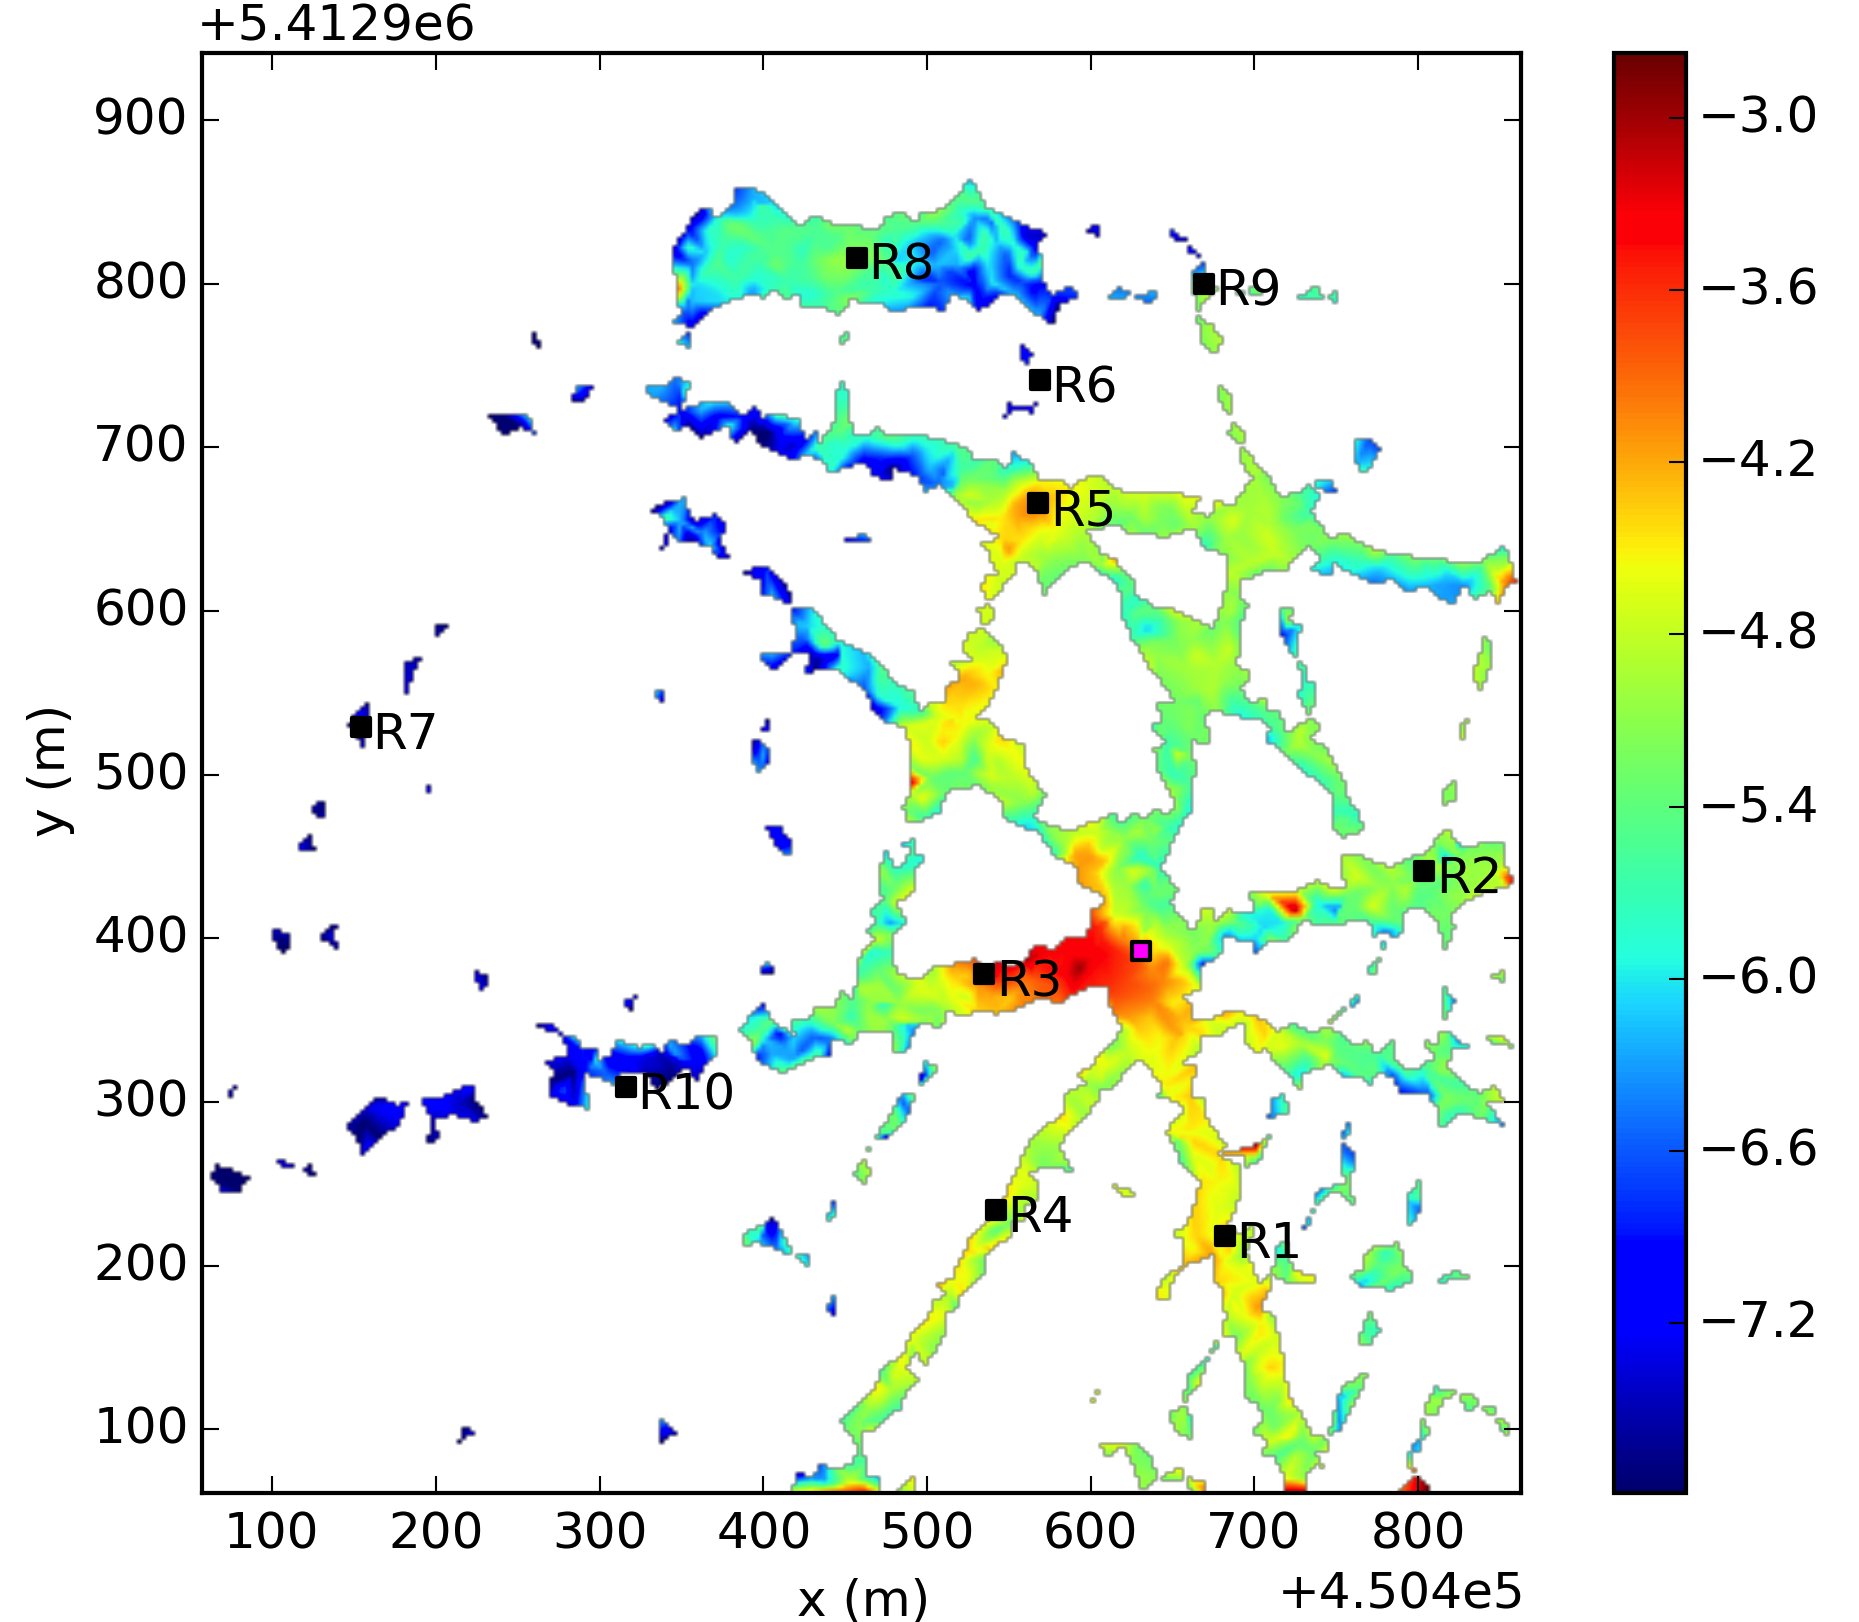
\includegraphics[width=1\textwidth]{opera_carte_fitting.png}
		\caption{}
		\label{opera_carte_fitting}
	\end{subfigure}%
	\begin{subfigure}[t]{0.5\textwidth}
		\centering
		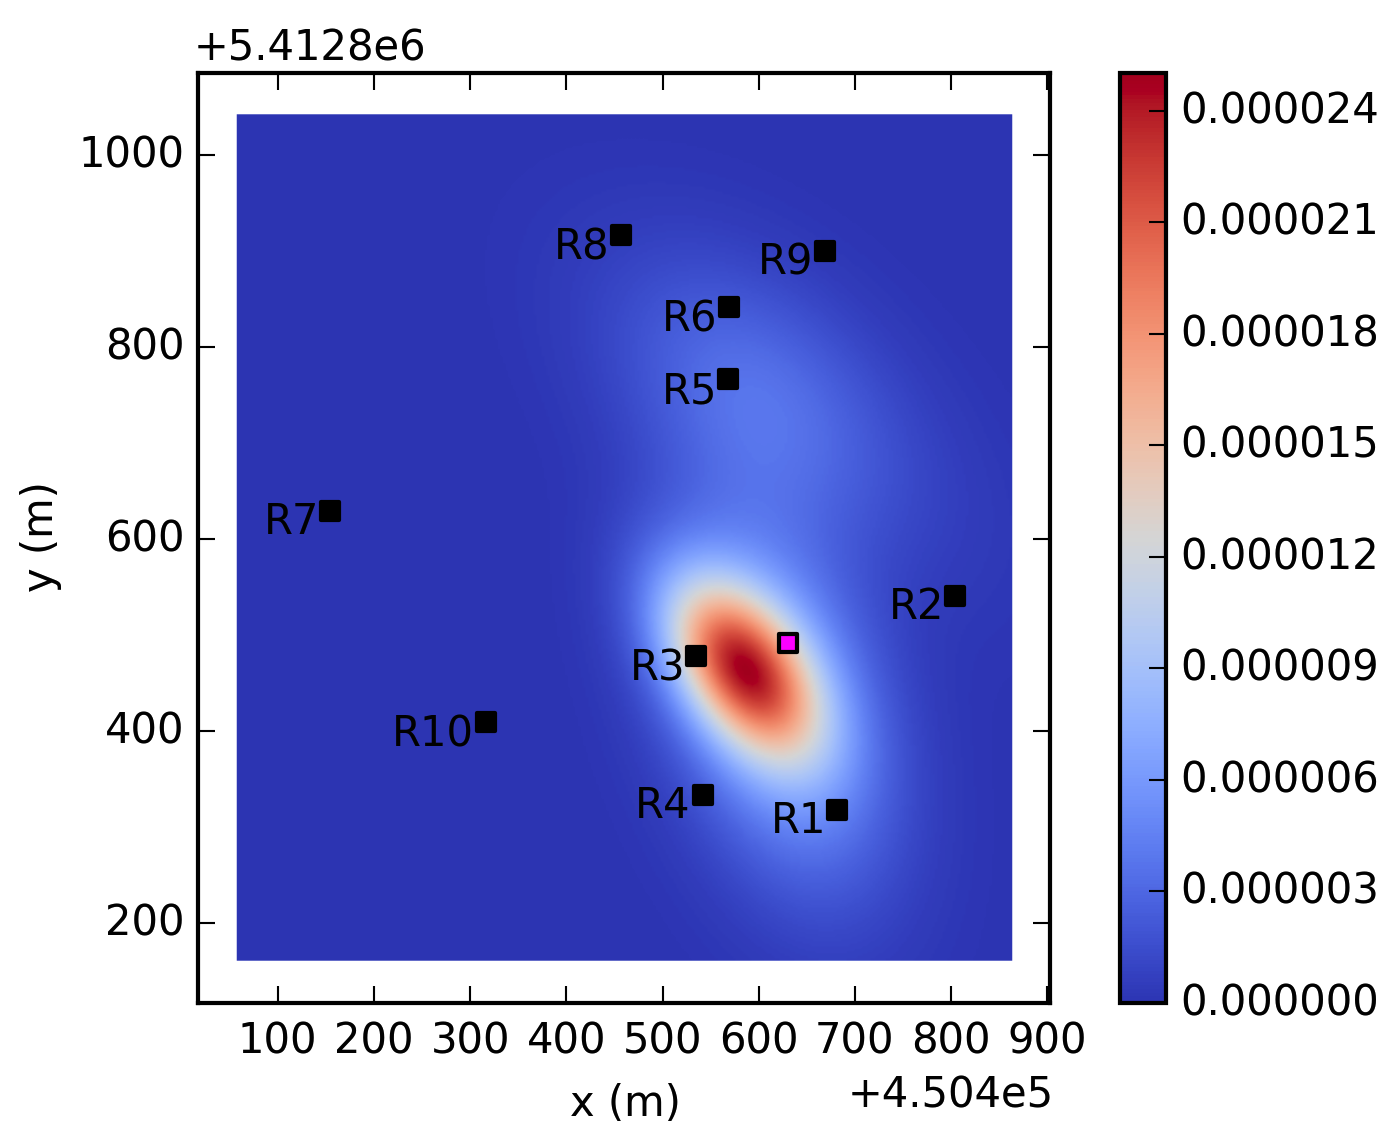
\includegraphics[width=1\textwidth]{opera_resultat_fitting.png}
		\caption{}
		\label{opera_resultat_fitting}
	\end{subfigure}
	\caption{Illustration de la procédure d'initialisation optimisée de la loi de proposition, avec la carte des rétro-concentrations (gauche) et la densité de probabilité suivant les paramètres initialisés (à droite)}
	\label{fig_opera_fitting}
	
\end{figure}

\subsection{Résultats}

La figure \ref{fig_opera_amis} présente le résultat d'un \textit{run} de 10 itérations de l'AMIS avec 100 particules tirées par itération, avec une initialisation optimisée et en utilisant les paramètres $\varObs = 7 \times 10^{-2}$ et $\varQ = 5\times 10^7$. Comme on pouvait s'y attendre après l'ajustement initial de la loi de proposition, la localisation de la source est correcte, de même, le profil de rejet est bien estimé. Les scores d'erreur sont de $r_d = 0.048$ pour l'estimation ponctuelle et $Err(\widetilde{\VecMu}_q) = 628.974$ pour le débit.


\begin{figure}[h!]
	\centering
	\begin{subfigure}[t]{0.5\textwidth}
		\centering
		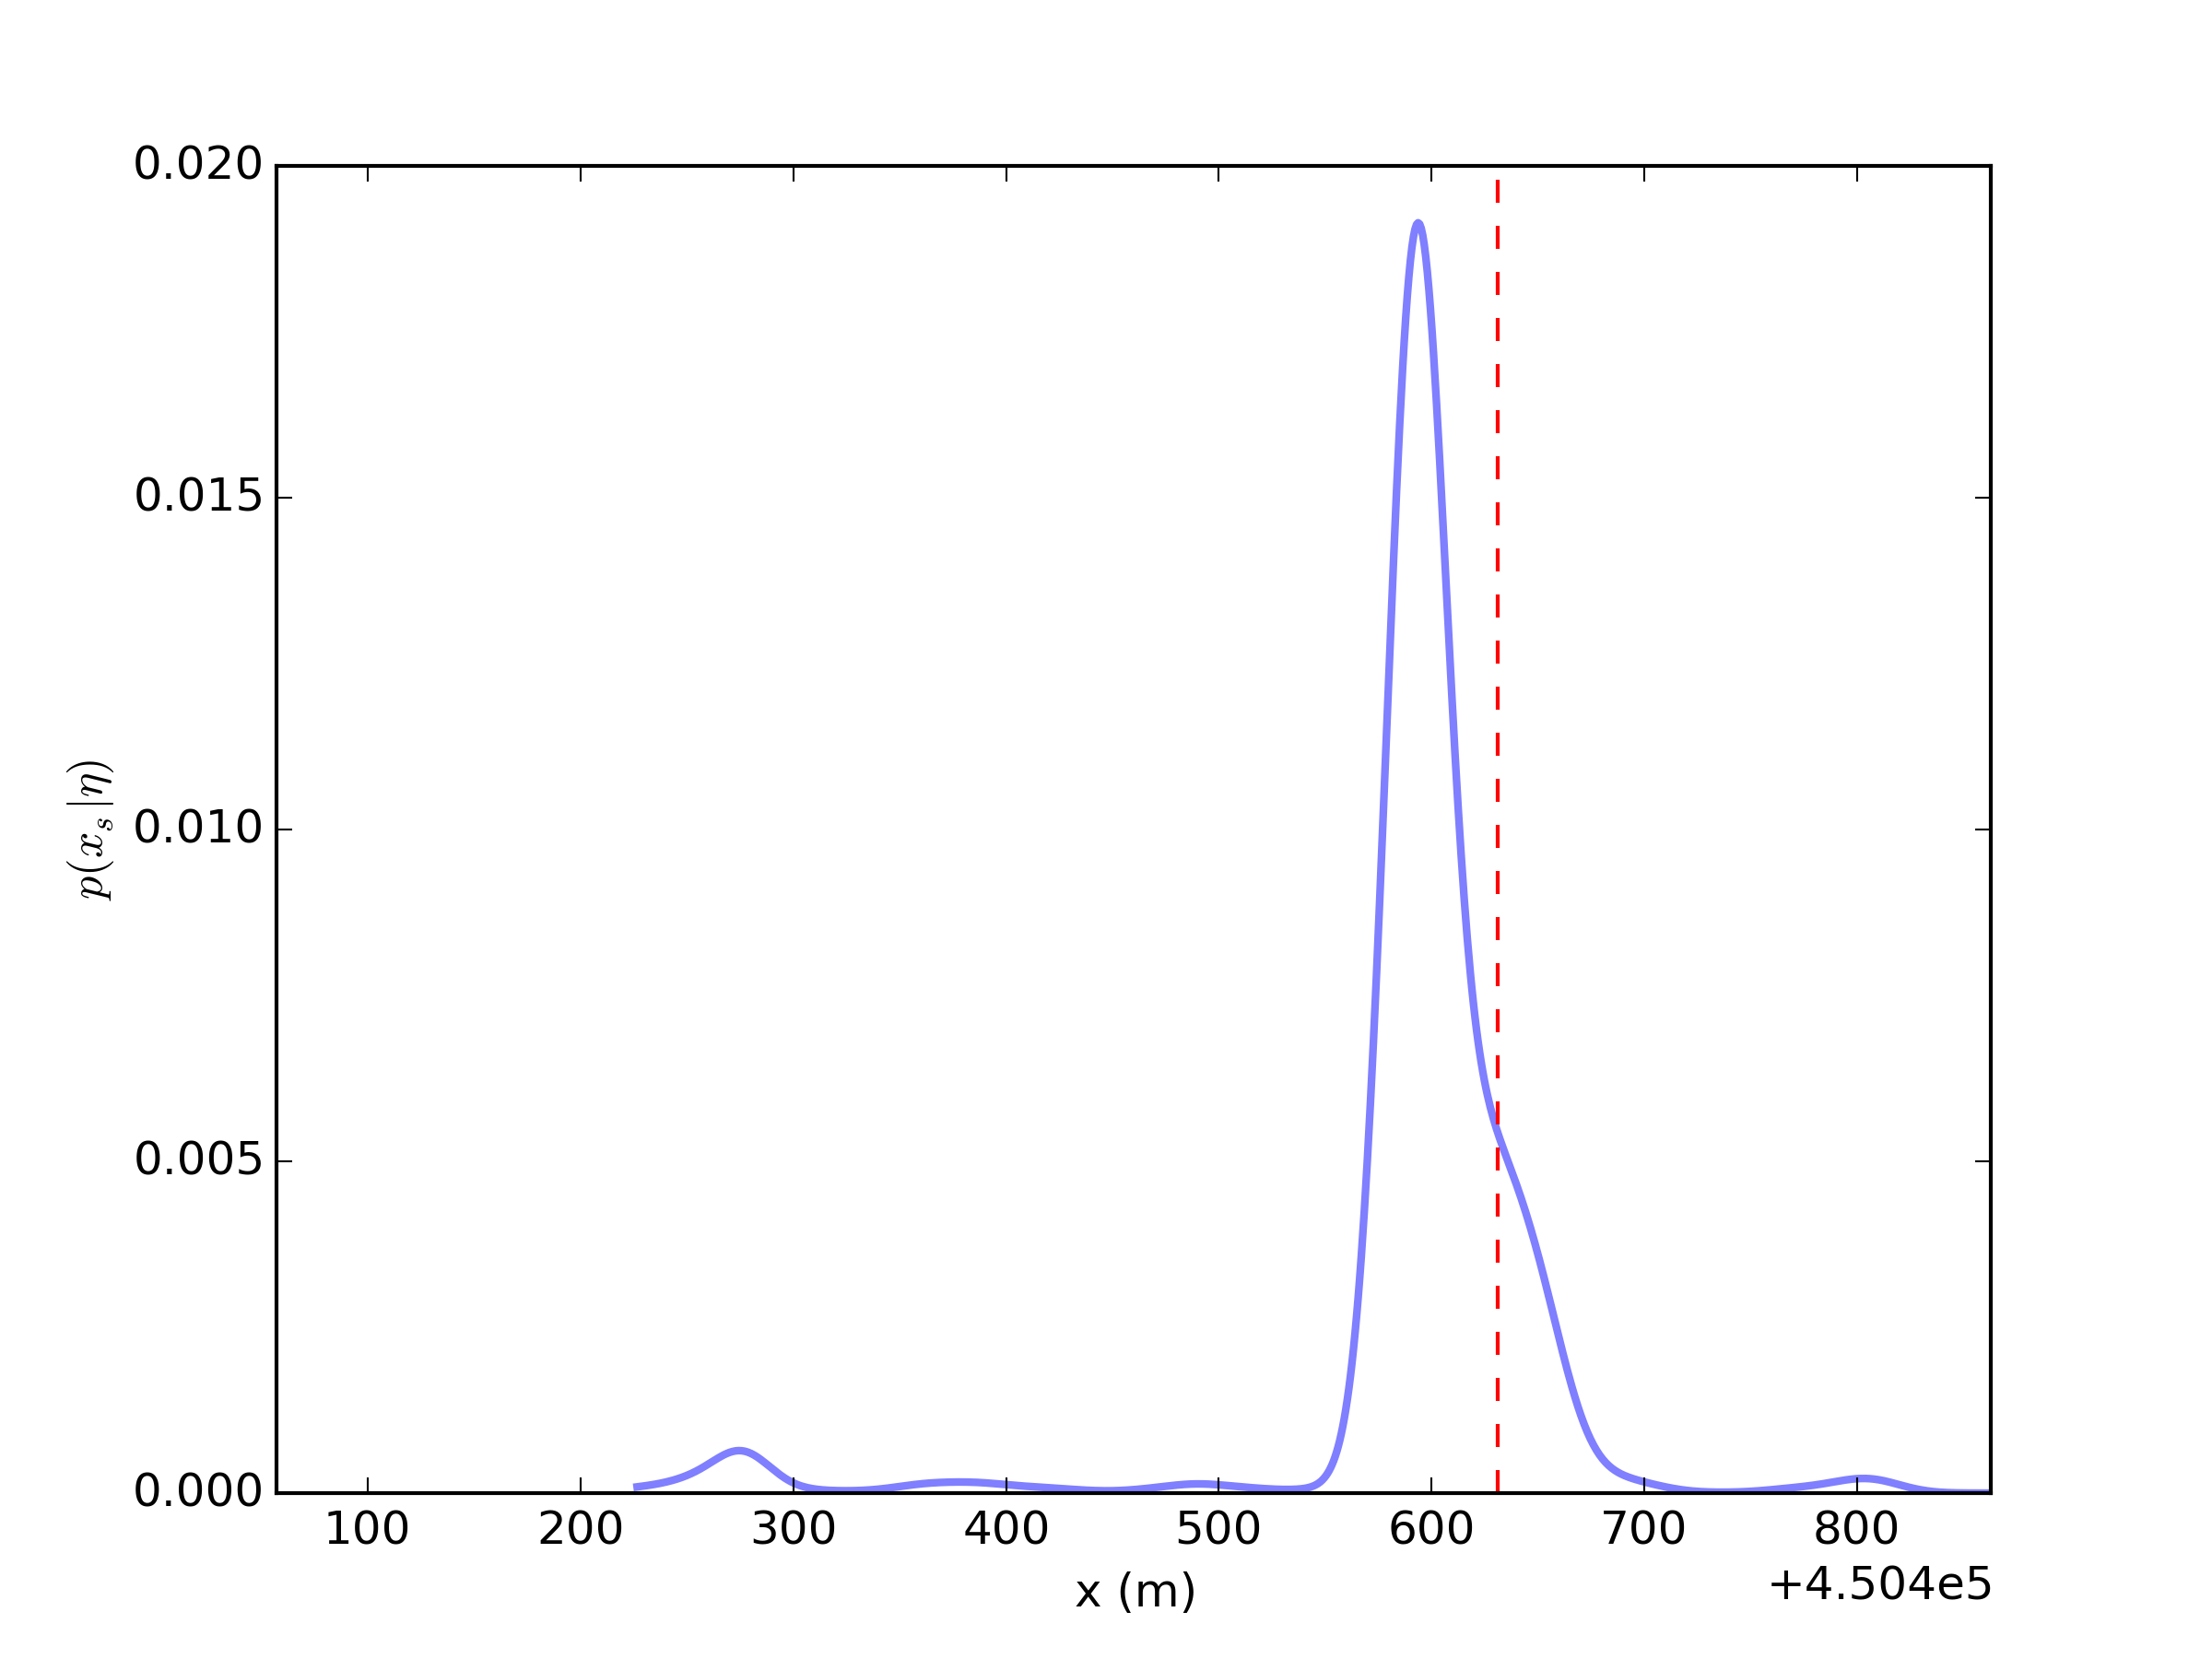
\includegraphics[width=1\textwidth]{opera_amis_kde_x.png}
		\caption{Position en $x$}
		\label{opera_amis_x}
	\end{subfigure}%
	\begin{subfigure}[t]{0.5\textwidth}
		\centering
		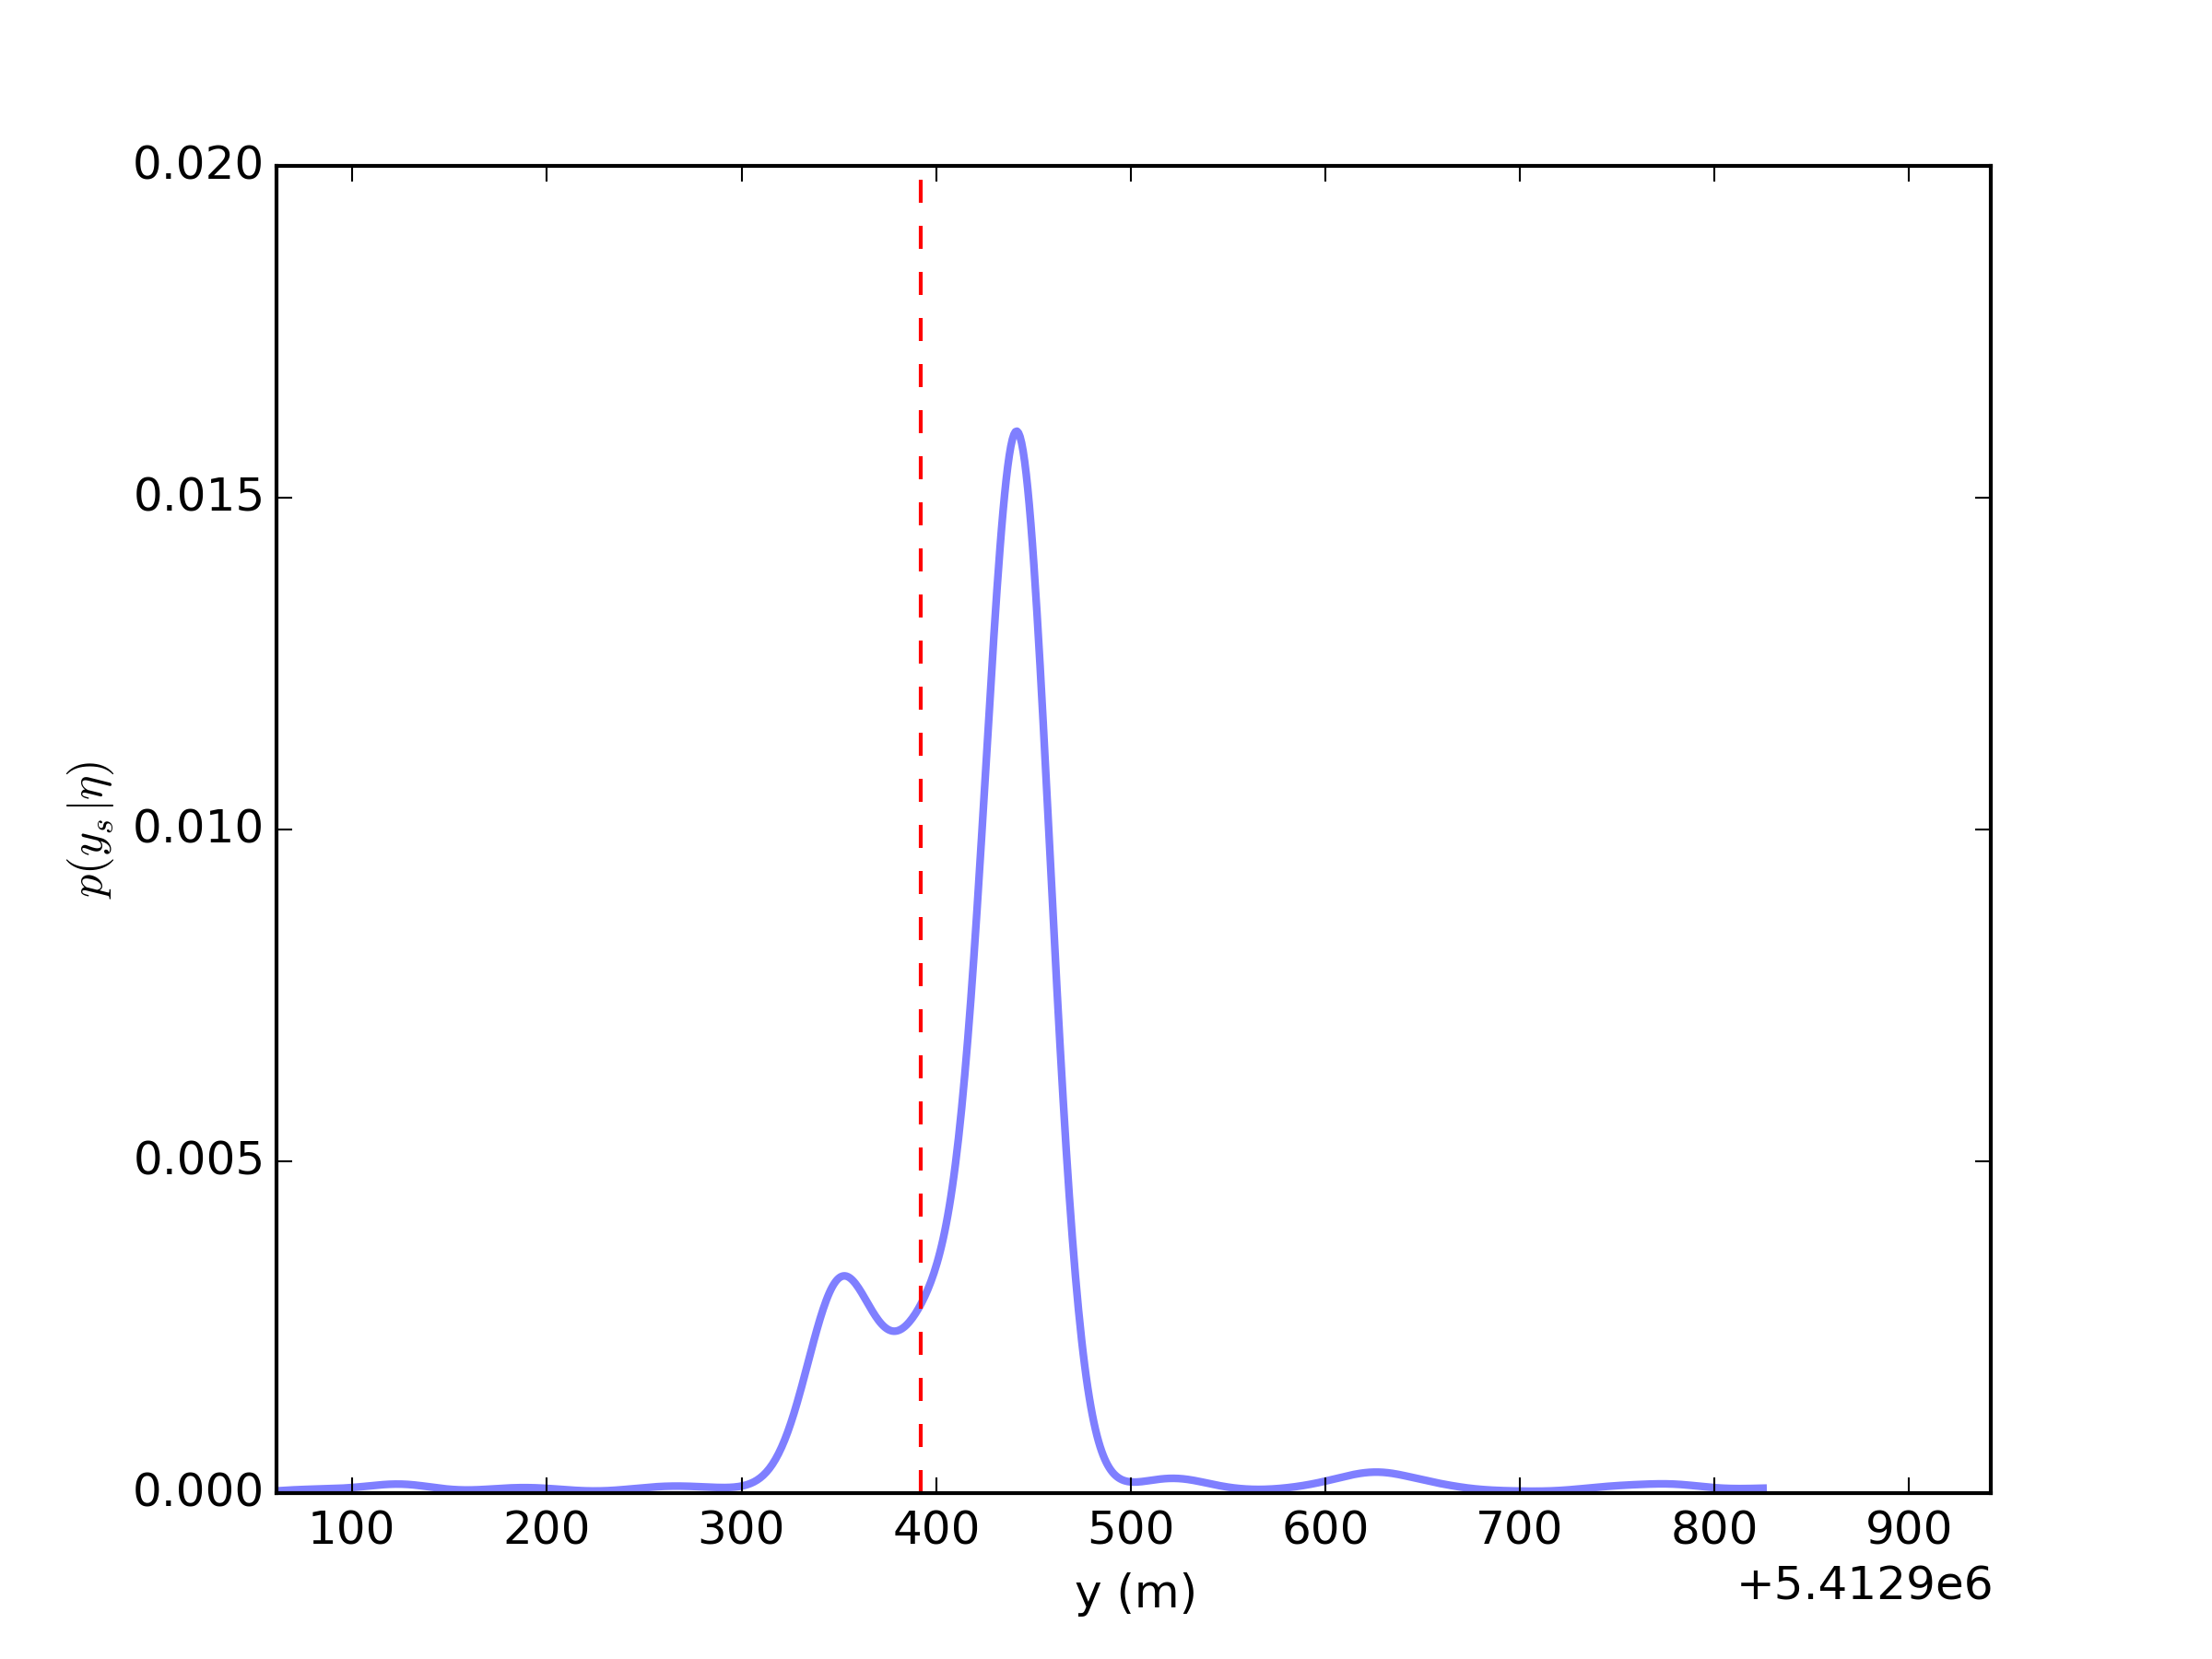
\includegraphics[width=1\textwidth]{opera_amis_kde_y.png}
		\caption{Position en $y$}
		\label{opera_amis_y}
	\end{subfigure}
	\begin{subfigure}[t]{0.65\textwidth}
		\centering
		\includegraphics[width=1\textwidth]{opera_amis_q.png}
		\caption{Profil d'émission avec intervalle de confiance à  $\pm 2 \widetilde{\sigma}_q^2$ (gris)}
		\label{opera_amis_q}
	\end{subfigure} 
	\caption{Résultats de l'algorithme d'estimation sur le cas-test Opéra avec une initialisation optimisée}
	\label{fig_opera_amis}
\end{figure}

Bien que l'initialisation optimisée ait permis une bonne reconstruction du terme source, il est à noter que la procédure d'échantillonnage depuis la loi de proposition elle-même n'est pas complètement efficace dans le cas urbain. En effet, durant cette procédure, un certain nombre de particules est tiré à l'intérieur des bâtiments, or une des hypothèses de départ stipule que la source se situe en extérieur. Pour toute particule tirée dans un bâtiment, la rétro-concentration qui lui est attribuée est automatiquement nulle, ce qui par conséquent réduit considérablement le nombre de particules pouvant avoir un poids d'importance représentatif, et réduit ainsi l'efficacité du processus d'échantillonnage d'importance. 

Une solution envisagée a été d'implémenter le ré-échantillonnage systématique de toute particule tirée dans un bâtiment, tant que celle-ci n'est pas en extérieur. Cependant, une telle démarche peut grandement allonger le temps de calcul, car la surface couverte par les bâtiments est supérieure à celle en extérieur sur le domaine. De plus, l'échantillon obtenu après ces ré-échantillonnages ne représente plus mathématiquement la loi de proposition, et fausse donc le déroulement de l'algorithme d'estimation. 

Une autre alternative plus simple consisterait à augmenter le nombre de particules par itération, afin d'accroître la proportion d'échantillons tirés en extérieur, ce qui n'impacte pas directement le temps de calcul du fait de l'implémentation optimale de l'opération de lecture des fichiers binaires. 

%Il a donc fallu chercher un moyen d'initialiser la loi de proposition pour l'AMIS de façon plus judicieuse qu'une simple hypothèse de répartition uniforme des particules sur le domaine. Une initialisation optimisée permet en effet d'explorer des zones potentiellement intéressantes plus rapidement, augmentant l'efficacité de l'algorithme d'estimation. \\

%Comme dans notre cas on a choisi une loi de proposition de type mixture de $D$ gaussiennes $\varphi_1, \dots, \varphi_D$, on va chercher à estimer les moyennes $\left(\VecMu_d\right)_{1:d}$ et les matrices de covariance $\left(\MatSigma_d\right)_{1:d}$ de chacune de ces composantes, ainsi que leurs facteurs d'influence $\left(\alpha_d\right)_{1:d}$. 

%Pour cela, in utilise les résultats issus d'un \textit{run} de rétro-propagation: suivant un modèle de dispersion dual tel que RetroSPRAY, on construit une série de cartes des concentrations conjuguées sur tout le domaine, en transformant les capteurs en rétro-sources et en utilisant les concentrations mesurées comme valeurs de rétro-émission. Une fois ces cartes créées, elles sont vues comme des ébauches des densités de probabilité sur la position de la source pour différents temps d'émission. L'objectif est alors de caler les paramètres $\left(\alpha_d, \VecMu_d,\MatSigma_d \right)_{1:D}$ sur ces densités.\\

%On part de l'instant d'observation $t_0$ qui est celui où la concentration la plus élevée a été observée. On définit ensuite un instant $t_{RP}$ qui correspond à l'instant final de la rétro-propagation, avec $t_{RP} < t_0$.  



